\documentclass[12pt]{article}
\usepackage[margin=1in]{geometry}
\usepackage{setspace}
\onehalfspacing
\usepackage{graphicx}
\usepackage{booktabs}
\usepackage{amsmath}
\usepackage{hyperref}
\usepackage{float}

\title{BANA290 --- AI Lab: Propensity Score Matching Analysis\\[6pt]
\large Interpretation of AI Adoption Effects on Revenue Growth}
\author{AI Lab Report}
\date{April 2026}

\begin{document}
\maketitle

\section{Overview}

This report analyzes whether AI adoption causally impacts year-over-year (YoY) revenue growth among 114 North American fintech firms scraped from the BANA290 assignment directory. After scraping and cleaning the data---standardizing revenue figures, parsing R\&D spend, and mapping AI program labels to a binary treatment variable---79 firms with complete records were retained for analysis. Of these, 41 firms were classified as AI adopters (treatment) and 38 as non-adopters (control).

\section{Baseline OLS Results}

A naive OLS regression of \texttt{REV\_GROWTH} on \texttt{AI\_ADOPTED} yielded a coefficient of \textbf{5.58 percentage points} ($p < 0.001$, $R^2 = 0.43$), suggesting AI-adopting firms grew substantially faster. However, this estimate is likely confounded by observable firm characteristics---larger, better-funded, and more digitally mature firms may simultaneously adopt AI \emph{and} grow faster.

\begin{table}[H]
\centering
\caption{Baseline OLS: Revenue Growth $\sim$ AI Adoption}
\begin{tabular}{lcccc}
\toprule
 & Coefficient & Std.\ Error & $t$-stat & $p$-value \\
\midrule
Intercept & 8.4763 & 0.527 & 16.07 & $< 0.001$ \\
AI\_ADOPTED & 5.5798 & 0.732 & 7.62 & $< 0.001$ \\
\bottomrule
\end{tabular}
\end{table}

\section{Propensity Score Matching}

\subsection{How did the AI coefficient change after applying PSM?}

After estimating propensity scores via logistic regression on seven covariates (log revenue, team size, firm age, R\&D spend, digital sales percentage, compliance tier, and fraud exposure) and performing one-to-one nearest-neighbor matching, the AI adoption coefficient \textbf{decreased from 5.58 to 3.52 percentage points}---a reduction of approximately 37\%. The PSM-adjusted effect remains statistically significant ($p < 0.001$), indicating that AI adoption is still associated with meaningfully higher revenue growth even after accounting for selection on observables.

\begin{table}[H]
\centering
\caption{PSM-Adjusted OLS: Revenue Growth $\sim$ AI Adoption (Matched Sample, $n = 82$)}
\begin{tabular}{lcccc}
\toprule
 & Coefficient & Std.\ Error & $t$-stat & $p$-value \\
\midrule
Intercept & 10.5390 & 0.490 & 21.50 & $< 0.001$ \\
AI\_ADOPTED & 3.5171 & 0.693 & 5.07 & $< 0.001$ \\
\bottomrule
\end{tabular}
\end{table}

\subsection{What does this shift suggest about selection bias?}

The 2.06-percentage-point drop reveals substantial \textbf{upward selection bias} in the naive estimate. Firms that adopt AI tend to be larger, invest more in R\&D, and have higher digital sales penetration---characteristics that independently drive revenue growth. The naive OLS conflated these pre-existing advantages with the treatment effect of AI itself. By matching adopters with observationally similar non-adopters, PSM isolates a more credible---though still correlational---estimate of AI's incremental contribution. This finding underscores that many ``AI impact stories'' in industry reporting likely overstate causal effects by ignoring the systematic differences between firms that choose to invest in AI and those that do not.

\subsection{Common Support}

Figure~\ref{fig:common_support} displays the propensity score distributions for treated and control groups. The histograms exhibit substantial overlap across the $[0.2, 0.8]$ range, confirming that the common support assumption is reasonably satisfied. This overlap ensures that for nearly every AI-adopting firm, a comparable non-adopter exists with a similar likelihood of treatment, making matched comparisons credible.

\begin{figure}[H]
\centering
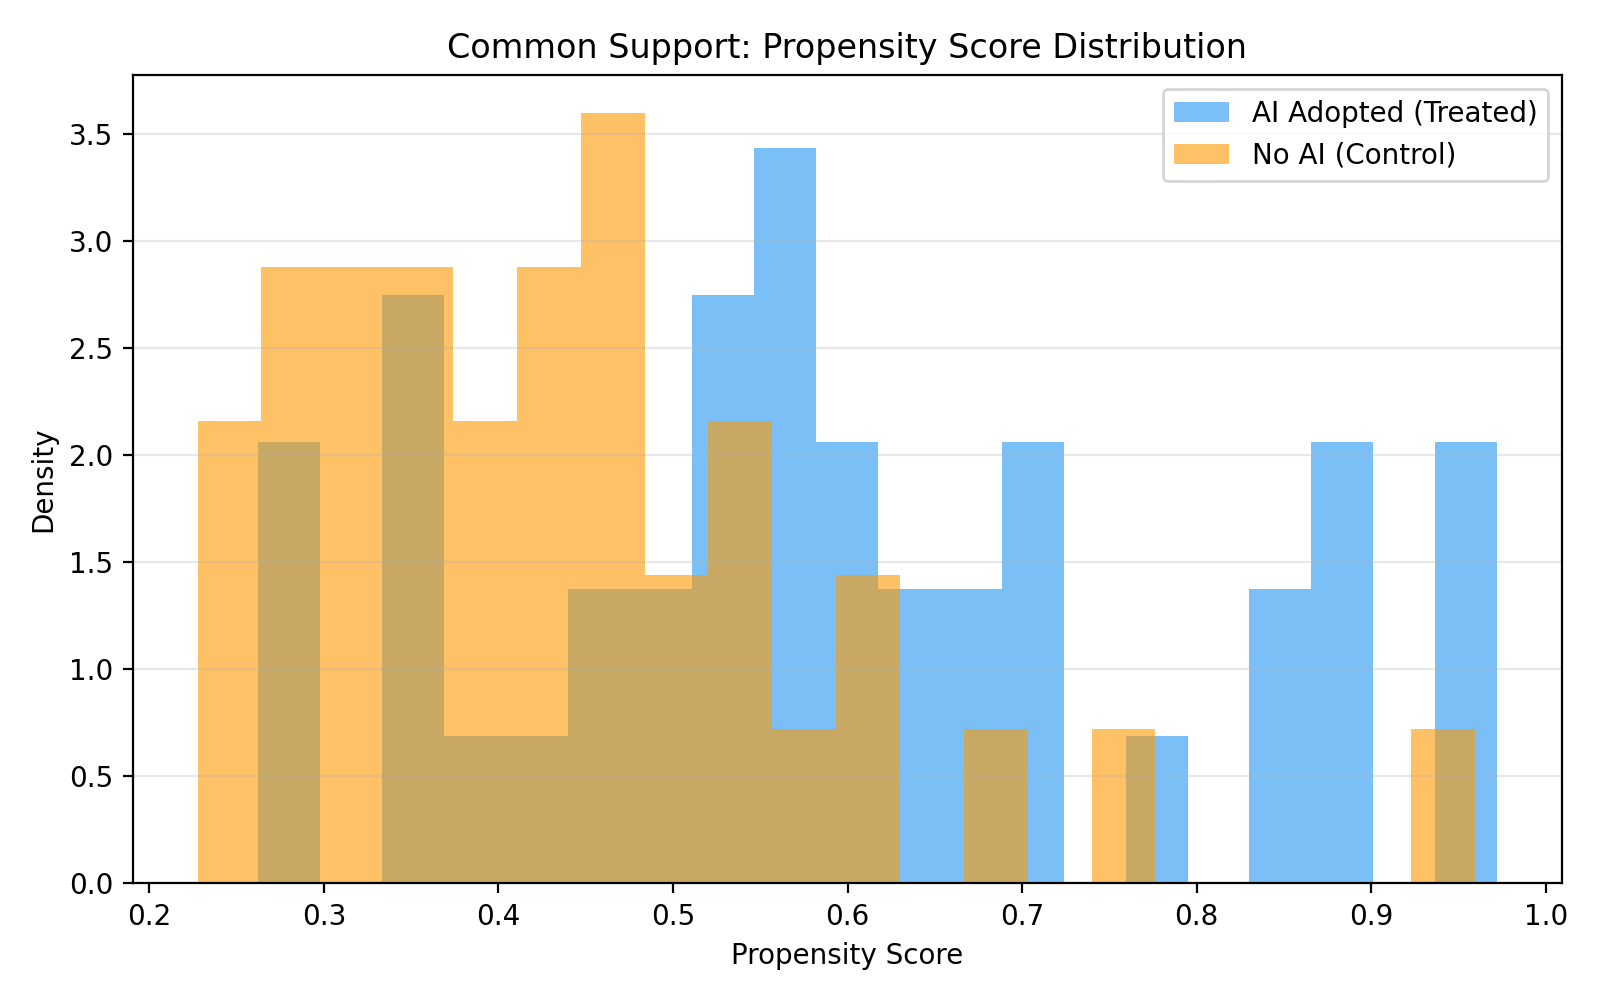
\includegraphics[width=0.85\textwidth]{fig_common_support.png}
\caption{Common Support: Propensity score distributions for AI adopters (blue) and non-adopters (orange) show wide overlap.}
\label{fig:common_support}
\end{figure}

\subsection{Balancing Property}

Table~\ref{tab:smd} and Figure~\ref{fig:love} present the Standardized Mean Differences (SMD) before and after matching. Prior to matching, several covariates exhibited large imbalances: R\&D Spend (SMD = 0.73), log revenue (0.63), team size (0.52), digital sales (0.55), and fraud exposure (0.50)---all well above the conventional 0.10 threshold. After nearest-neighbor matching, all covariates fell to $|$SMD$|$ $\leq$ 0.28, with most below 0.10. This confirms that matching successfully balanced the treatment and control groups on observed characteristics, validating the balancing property.

\begin{table}[H]
\centering
\caption{Standardized Mean Differences Before and After Matching}
\label{tab:smd}
\begin{tabular}{lcc}
\toprule
Covariate & SMD (Before) & SMD (After) \\
\midrule
LOG\_REV & 0.6318 & $-0.2759$ \\
TEAM\_SIZE & 0.5216 & $-0.0750$ \\
FIRM\_AGE & 0.2010 & 0.0822 \\
RD\_SPEND & 0.7340 & $-0.0720$ \\
DIGITAL\_SALES & 0.5451 & $-0.0158$ \\
COMPLIANCE\_TIER & $-0.1036$ & 0.0000 \\
FRAUD\_EXPOSURE & 0.4969 & $-0.0269$ \\
\bottomrule
\end{tabular}
\end{table}

\begin{figure}[H]
\centering
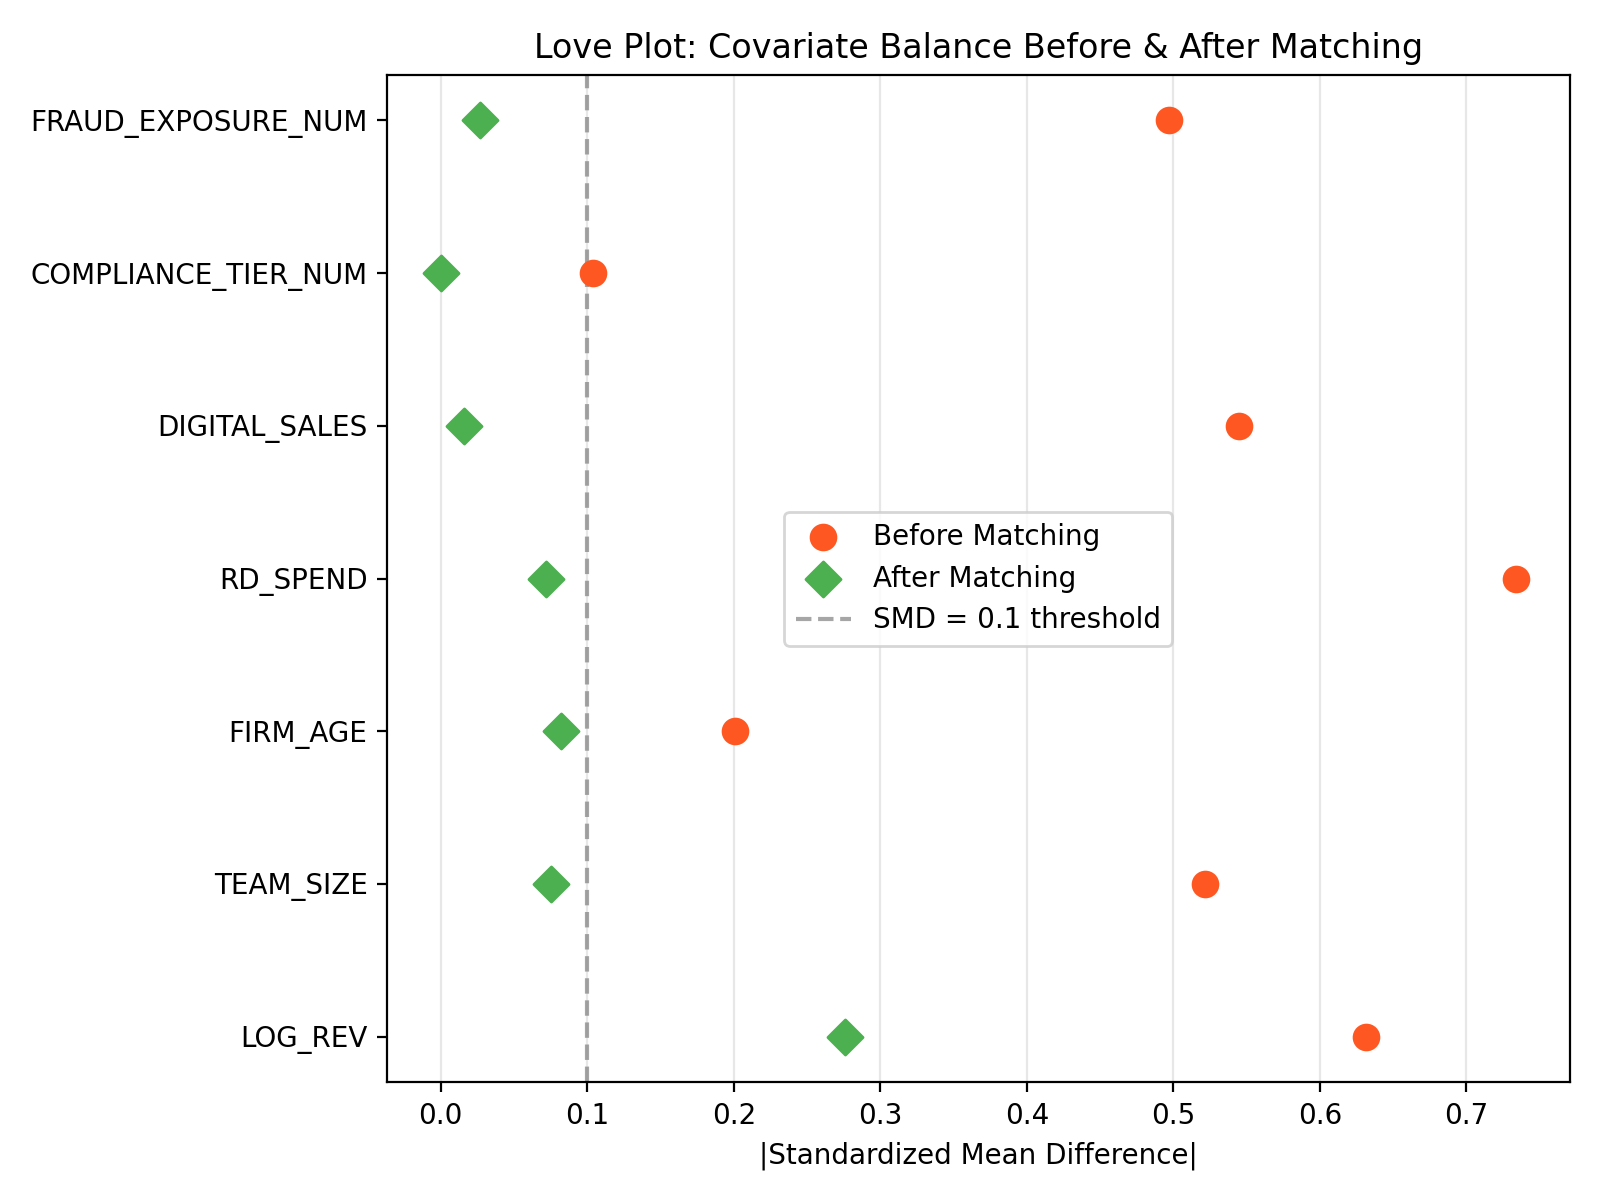
\includegraphics[width=0.85\textwidth]{fig_love_plot.png}
\caption{Love Plot: Absolute SMD values before (red circles) and after (green diamonds) matching. The dashed line marks the 0.1 threshold.}
\label{fig:love}
\end{figure}

\section{Conclusion}

Propensity score matching reduced the estimated AI adoption effect on revenue growth by roughly 37\%, from 5.58 to 3.52 percentage points. The remaining effect is still statistically significant, suggesting a genuine positive association between AI adoption and growth---though unobserved confounders may still play a role. The common support and balancing diagnostics indicate that the PSM procedure was well-executed, lending credibility to the adjusted estimate.

\end{document}
